\section{Theory and experimental setup}
\subsection{Coordinate systems}
When operating a radio telescope, different coordinate systems can be used used to locate objects on the celestial sphere.
As explained in \cite{carroll_introduction_2007}, three main ones are used in astronomy:
\begin{itemize}
    \item The \textbf{Altitude-Azimuth} (Alt-Az) coordinate system is based on the observer's local horizon. The altitude $h$ is the angle measured from the horizon to the object along a circle which passes through the object itself and the point on the celestial sphere directly above the observer, i.e. the zenith. The azimuth $a$ is the angle measured along the horizon eastward from north to the circle used for the measure of altitude.
    \item The \textbf{Right Ascension-Declination} (Ra-Dec) coordinate system, also called \textbf{Equatorial}, is based on the latitude-longitude system of Earth, thus removing the dependency on the position of the observer, but does not participate in the planet's rotation. Declination $\delta$ is the equivalent of latitude and measured in degrees north or south of the celestial equator. Right ascension $\alpha$ is analogous to longitude and is measured eastward along the celestial equator from the vernal equinox, i.e. the position of the Sun at Spring equinox, to the object's hour circle, i.e. the circle passing throught the object and the north celestial pole.
    \item The \textbf{Galactic} coordinate system is often used when studying the structure and kinematics of the Milky Way, exploiting the natural symmetry introduced by the existance of the Galactic disk. The intersection of the midplane of the Galaxy with the celestial sphere defines the Galactic equator. Galactic latitude $b$ is measured north or south of the Galactic equator along a circle which passes through the North Galactic Pole. Galactic longitude $l$ is measured east along the Galactic equator, starting from near the Galactic center to the point of intersection with the circle used to measure the latitude.
\end{itemize}
The methods of spherical trigonometry allow to convert between equatorial and Galactic coordinates \Cite{carroll_introduction_2007}. To make the transformation from equatorial to Galactic (assuming epoch J2000.0):
\begin{align}
    \sin b &= \sin \deltaNGP \sin \delta + \cos \deltaNGP \cos \delta \cos (\alpha - \alphaNGP) \\
    \cos b \sin(\lNCP - l) &= \cos \delta \sin(\alpha - \alphaNGP) \\
    \cos b \cos (\lNCP - l) &= \cos \deltaNGP \sin \delta - \sin \deltaNGP \cos \delta \cos(\alpha - \alphaNGP)
\end{align}
To make the reverse transformation from Galactic to equatorial (again assuming epoch J2000.0):
\begin{align}
    \sin \delta &= \sin \deltaNGP \sin b + \cos \deltaNGP \cos b \cos (\lNCP - l) \\
    \cos \delta \sin(\alpha - \alphaNGP) &= \cos b \sin(\lNCP - l) \\
    \cos \delta \sin(\alpha - \alphaNGP) &= \cos \deltaNGP \sin b - \sin \deltaNGP \cos b \cos (\lNCP - l)
\end{align}
Where $\alphaNGP = 12^{\text{h}} 51^{\text{m}} 26.28^{\text{s}}$ and $\deltaNGP = 28^{\circ}7' 41.7''$ are the J2000.0 equatorial coordinates of the north Galactic pole ($b = 90^{\circ}$) and $\lNCP = 123^{\circ} 55' 55.2''$ is the J2000.0 Galactic longitude of the north celestial pole.

\subsection{Sources of radio emissions}
Because of Earth's atmosphere, only two ranges of frequencies are completely open for the observation from the ground of electromagnetic waves coming from space: the optical window, which ranges from ??? to ??? and is studied through optical telescopes, and the wider radio window, which ranges from ??? to ??? and is instead the focus of radio astronomy.

Radio emissions originate from a broad range of phenomena.
A distinction must be made between physical processes which produce continuous radiation over a wider frequency range (mainly thermal processes and synchrotron radiation) and those that result in radiation only in a narrow frequency band, i.e.\ a \emph{spectral line} \cite{lauterbach_radio_2022}.
\begin{itemize}
    \item Thermal radiation is the process by which any body with non-zero temperature radiates electromagnetic waves. It is commonly modelled by the continuous black-body radiation of Planck's law \cite{carroll_introduction_2007}.
    \item Synchrotron emission originates instead from relativistic electrons spiraling along magnetic field lines \cite{maoz_astrophysics_2016}.
    \item Line sources emit or absorb electromagnetic waves only at very specific frequencies, associated with a transition between states of the electrons in the atomic shell.
\end{itemize}

\subsection{The hydrogen 21 cm line}
An example of spectral line is the 21 cm radiation of atomic hydrogen.
Neutral hydrogen does not emit any radiation in the visible spectrum, but it is possible to detect its presence in the interstellar medium (ISM) through the observation of radio waves.
When not excited, neutral hydrogen can exist in two states: either the electron and proton spins are aligned (state $F=1$), or they're opposite (state $F=0$).
Because of the interaction between the nucleus magnetic dipole moment and the electron orbital magnetic field, these two states have a very small difference in energy of $\Delta E = 5.88$ \si{\micro\electronvolt} (a splitting known as \emph{hyperfine structure} of the ground state) \cite{lauterbach_radio_2022}.
When transitioning from $F=1$ to $F=0$, a photon frequency of \mbox{$\nu_H = 1.420405751768$ GHz} gets emitted, corresponding to a wavelength of \mbox{$\lambda_H = 21.106114054160$ cm} in vacuum \cite{hellwig_measurement_1970}. This value is known very precisely, up to $10^{-12}$ Hz.
While this transition is exceptionally rare, with an average lifetime of about $11$ million years between transitions, and hydrogen density is low ($\sim 1$ cm$^{-3}$), its abundance and the very long lines of sight in the ISM allow radioastronomers to detect its presence in the Universe \cite{burke_introduction_2013}.

\subsection{Estimating the velocity field of the Milky Way}
Studying the H21 cm radiation allows us to derive the relative velocity of interstellar medium and therefore of other parts of the Milky Way or even other galaxies.
In fact, when an observer moves relative to a wave source, the frequency of the wave perceived by the observer is different from the emitted wave, according to what is called the Doppler effect.
The observed frequency $\nu_O$ is linked to the source frequency $\nu_S$ by \hl{[source stp Matteo c'est lequel de tes bouquins lmao]}:
\begin{equation}
    \nu_O = \frac{c - v_O}{c + v_S} \nu_S
    \label{eq:doppler_general}
\end{equation}
where $c$ is the speed of the wave, in this case the speed of light, $v_O$ is the speed of the observer, and $v_S$ is the speed of the source.
Only the components of velocity parallel to the axis connecting the source and the observer are taken into account, since we only consider relative velocity.

As shown in \autoref{fig:doppler_galaxy}, this effect can be used in astronomy to estimate the speed of distant objects, as the Doppler effect also applies to electromagnetic waves.
\begin{figure}[htbp]
    \centering
    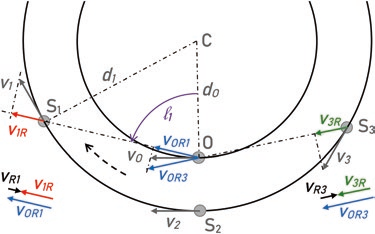
\includegraphics[width=0.6\linewidth]{figures/doppler_galaxy.png}
    \caption{The Doppler effect in the galaxy. $O$ reprents the observers position, $C$ the center of the Galaxy and $S_1$ the source of radiowaves. $v_{1R}$ and $v_{OR1}$ are the velocities taken into account for the Doppler effect. \cite{lauterbach_radio_2022}}
    \label{fig:doppler_galaxy}
\end{figure}
When observing the radio signal from distant hydrogen clouds in the Milky Way, the angular speed of the outer branches of the Milky Way can be calculated by the Doppler shift of the H$21$ cm line, whose frequency is known very precisely [citation].
In the reference frame where the observer is at rest $v_O = 0$, and knowing the source and observed frequencies, the angular speed of the distant part of the galaxy can be found to be, using \autoref{eq:doppler_general}
\begin{equation}
    v_S = c \frac{\nu_S - \nu_O}{\nu_O} \qquad \textrm{OR IF NOT IN REST FRAME} \qquad v_S = \frac{\nu_S}{\nu_O}(c - v_O) - c
    \label{eq:doppler}
\end{equation}

\subsection{The VEGA Small Radio Telescope}
The Very Elegant Galactic Antenna (VEGA) was built in 2022 by a group of students from the EPFL Section of Physics, following the design of MIT Haystack Observatory's Small Radio Telescope (SRT): an observational instrument of small size and built on a low budget, which focuses on the study of the 21 cm hydrogen radiation line \cite{interdisciplinary_project_2022}.

The operation of a radio telescope depends primarily on its receiving antenna, which serves a dual purpose: it concentrates the weak signals from the sources (in such a way that they can then be processed by the electronics) and it selects the area of the sky from which the signal is to be received \cite{lauterbach_radio_2022}.
Parabolic reflectors (also referred to as \emph{dishes}), are well suited for this purpose, as they concentrate the incident waves at the focal point, where the feed, i.e. the metal component which converts the radio waves into electric signals, is placed.
Both reflector and feed need to be suited to the desired operation of the telescope.
The dishes can have different diameters and focal lengths, and
feeds take several forms, each suited to a certain frequency range and dish geometry \cite{lauterbach_radio_2022}. 
A thorough study of these parameters is needed to reduce as much as possible the noise captured by the antenna, e.g. the thermal radiation from the ground below the parabola, at a physical temperature of 280-290 K, which can hit the feed from the area outside the reflector (the \emph{spillover}) \cite{burke_introduction_2013}.
In the case of VEGA, a parabola of diameter $1.86$ m, with a field of view of solid angle around $(7 \pm 1)^{\circ}$ is used to focus the signal on a copper helical feed of circumference $C = 21$ cm, radius $R = 3.34$ cm, pitch spacing $S = 5.25$ cm and pitch angle $\alpha = 14^{\circ}$ \cite{interdisciplinary_project_2022} \cite{rapport_interne_2024}. The antenna pattern, describing the sensibility of the instrument as a function of the incident angle, was simulated in \cite{rapport_interne_2024} using the GRASP software package. The results are shown in \autoref{fig:antenna_pattern}.

\begin{figure}[htbp]
    \begin{minipage}[t]{0.5\textwidth}
        \centering
        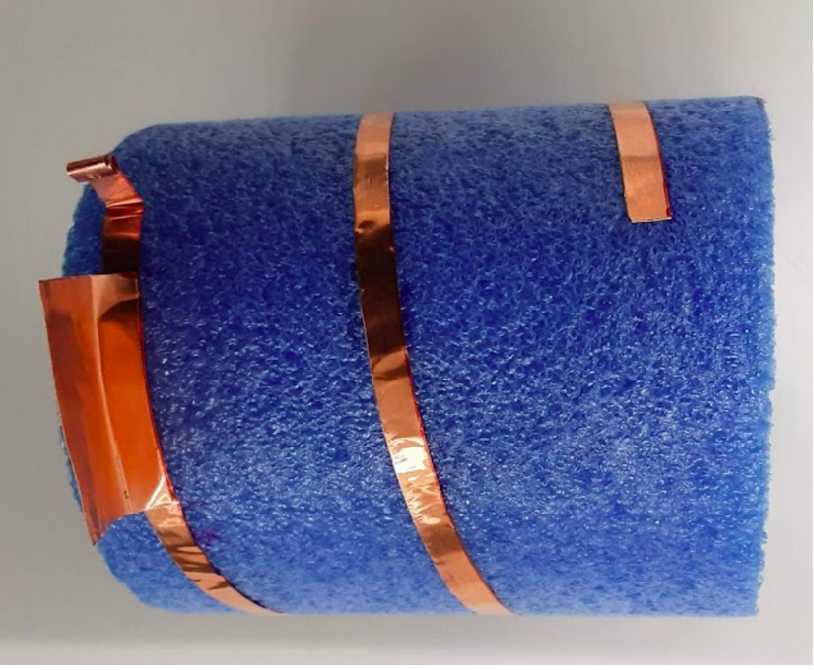
\includegraphics[width=8cm]{figures/antenna_photo.png}
        \caption{TEMP}
        \label{fig:antenna_photo}
    \end{minipage}
    \begin{minipage}[t]{0.5\textwidth}
        \centering
        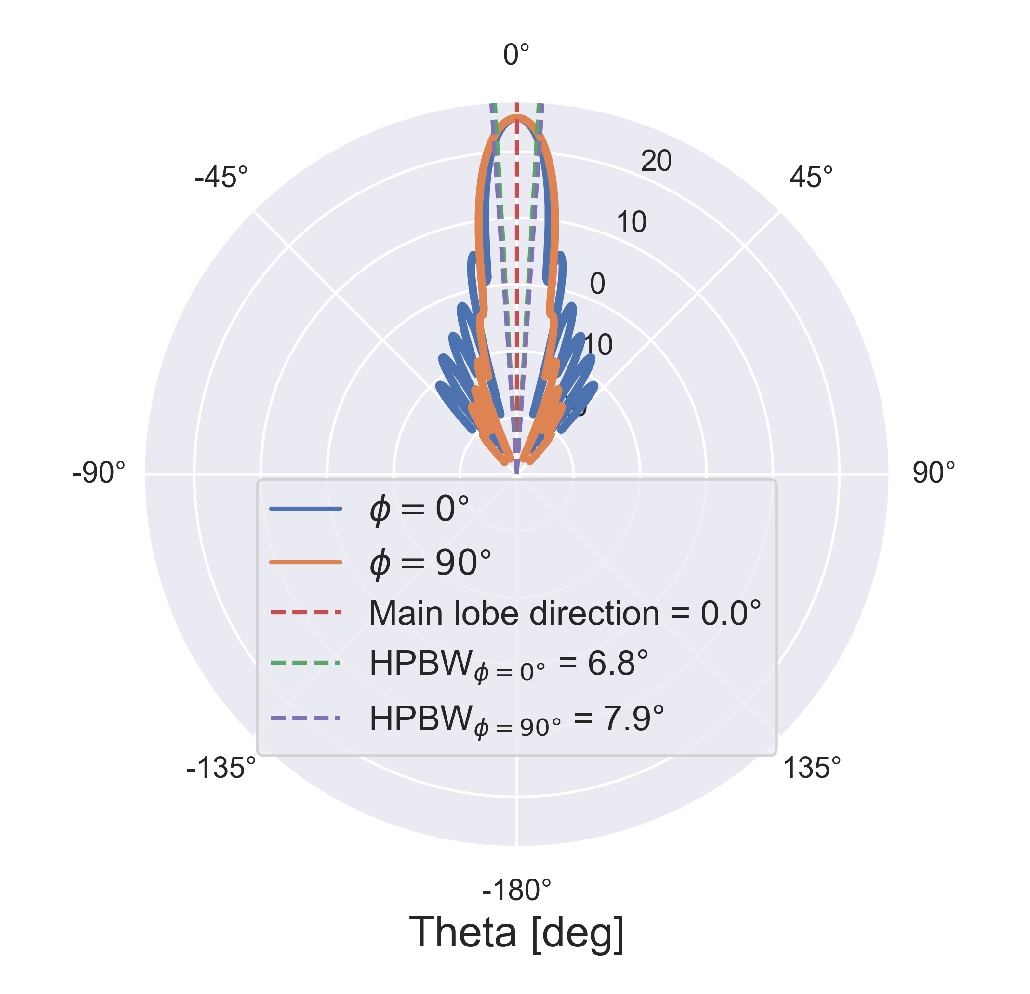
\includegraphics[width=8cm]{figures/antenna_pattern.png}
        \caption{Antenna pattern as simulated using the GRASP software package \cite{rapport_interne_2024}}
        \label{fig:antenna_pattern}
    \end{minipage}
\end{figure}

Once the electric signal is acquired, it passes first through a Low Noise Amplifier (LNA), composed of two amplifiers of total gain 42dB and a bandpass filter of frequency range 1376-1441 MHz, then a Bias Tee which suppresses the DC effects caused by the other components, and finally a second bandpass filter of frequency range 1395-1445 MHz \cite{interdisciplinary_project_2022}.
The signal, now amplified and limited to the desired frequency range, is digitized using an RTL2832U demodulator. 

